% !TEX root = ./SPP_IoTjournal.tex
\section{Simulations \label{sec:simulations}}
We now illustrate the proposed algorithm using a fifty-vehicle example. 

\subsection{Setup \label{sec:simSetup}}
Our goal is to simulate a scenario where UAVs are flying through an urban environment. This setup can be representative of many UAV applications, such as package delivery, aerial surveillance, etc. For this purpose, we use the city of San Francisco (SF), California, USA as our planning region, as shown in Figure \ref{fig:sf_setup}. Practically speaking, depending on the UAV density, it may be desirable to have smaller planning regions that together cover the SF area; however, such considerations are out of the scope of this paper.

\begin{figure}
  \centering
  \includegraphics[width=0.8\columnwidth]{"figs/sf_setup"}
  \caption{Simulation setup. A \SI{25}{\km\squared} area of San Francisco city is used as the state-space for vehicles. STP vehicles originate from the Blue star and go to one of the four destinations, denoted by circles. Tall buildings in the downtown area are used as static obstacles, represented by the black contours.}
  \label{fig:sf_setup}
\end{figure}
Each box in Figure \ref{fig:sf_setup} represents a \SI{500}{\m} $\times$ \SI{500}{\m} area of SF. The origin point for the vehicles is denoted by the Blue star. Four different areas in the city are chosen as the destinations for the vehicles. Mathematically, the target sets $\targetset_i$ of the vehicles are circles of radius $r$ in the position space, i.e. each vehicle is trying to reach some desired set of positions. In terms of the state space $\state_i$, the target sets are defined as $\targetset_i = \{\state_i: \|\pos_i - c_i\|_2 \le 100 \text{m}\}$, where $c_i$ are centers of the target circles. The four targets are represented by four circles in Figure \ref{fig:sf_setup}. The destination of each vehicle is chosen randomly from these four destinations. Finally, tall buildings in downtown San Francisco are used as static obstacles, denoted by black contours in Figure \ref{fig:sf_setup}. We use the following dynamics for each vehicle:
\begin{equation}
\label{eq:dyn_i}
\begin{aligned}
\dot{\pos}_{x,i} &= v_i \cos \theta_i + d_{x,i} \\
\dot{\pos}_{y,i} &= v_i \sin \theta_i + d_{y,i}\\
\dot{\theta}_i &= \omega_i, \\
\underline{v} \le v_i \le \bar{v}, & ~|\omega_i| \le \bar{\omega}, ~\|(d_{x,i}, d_{y,i}) \|_2 \le d_{r},
\end{aligned}
\end{equation}
\noindent where $\state_i = (\pos_{x,i}, \pos_{y,i}, \theta_i)$ is the state of vehicle $\veh_i$, $\pos_i = (\pos_{x,i}, \pos_{y,i})$ is the position and $\theta_i$ is the heading. $d = (d_{x,i}, d_{y,i})$ represents $\veh_i$'s disturbances, for example wind, that affect its position evolution. The control of $\veh_i$ is $u_i = (v_i, \omega_i)$, where $v_i$ is the speed of $\veh_i$ and $\omega_i$ is the turn rate; both controls have a lower and upper bound. To make our simulations as close as possible to real scenarios, we choose velocity and turn-rate bounds as $\underline{v} = $\SI{0}{\m\per\s}, $\bar{v} = $\SI{25}{\m\per\s}, $\bar\omega = $\SI{0}{\radian\per\s}, aligned with the modern UAV specifications \cite{UAVspecs1, UAVspecs2}. The disturbance bound is chosen as $d_{r} = $\SI{6}{\m\per\s}, which corresponds to \textit{moderate winds} on the Beaufort wind force scale \cite{Windscale}. Note that we have used same dynamics and input bounds across all vehicles for clarity of illustration; however, our method can easily handle more general systems of the form in which the vehicles have different control bounds and dynamics.

The goal of the vehicles is to reach their destinations while avoiding a collision with the other vehicles or the static obstacles. The vehicles also need to account for the possibility of the presence of an intruder for a maximum duration of $\iat = $\SI{10}{\s}, whose dynamics are given by \eqref{eq:dyn_i}. The joint state space of this fifty-vehicle system is 150-dimensional (150D); therefore, we assign a priority order to vehicles and solve the trajectory planning problem sequentially. For this simulation, we assign a random priority order to fifty vehicles and use the algorithm proposed in Section \ref{sec:intruder} to compute a separation between STP vehicles so that they do not collide with each other or the intruder. 

\subsection{Results \label{sec:simResults}}
In this section, we present the simulation results for $\nva = 3$; occasionally, we also compare the results for different values of $\nva$ to highlight some key points about the proposed algorithm. As per Algorithm \ref{alg:intruder_plan}, we begin with computing the avoid region $\brs^{\text{A}}_{i}(0, \iat)$. To compute the avoid region, relative dynamics between $\veh_i$ and $\veh_{\intr}$ are required. Given the dynamics in \eqref{eq:dyn_i}, the relative dynamics are given by \cite{Mitchell05}:
\begin{equation}
\label{eq:reldyn_i}
\begin{aligned}
\dot{\pos}_{x, \intr, i} &= v_{\intr} \cos \theta_{\intr, i} - v_i + \omega_i {\pos}_{y, \intr, i} + d_{x,i} + d_{x,\intr}\\
\dot{\pos}_{y, \intr, i} &= v_i \sin \theta_{\intr, i} - \omega_i {\pos}_{x, \intr, i} + d_{y,i} + d_{y,\intr}\\
\dot{\theta}_{\intr, i} &= \omega_{\intr} - \omega_i,
\end{aligned}
\end{equation}    
where $\state_{\intr, i} = (\pos_{x, \intr, i}, \pos_{y, \intr, i}, \theta_{\intr, i})$ is the relative state between $\veh_{\intr}$ and $\veh_i$. Given the relative dynamics, the avoid region can be computed using \eqref{eqn:avoidBRS}. For all the BRS and FRS computations in this simulation, we use Level Set Toolbox \cite{Mitchell07b}. Also, since the vehicle dynamics are same across all vehicles, we will omit the vehicle index from sets wherever applicable. The avoid region $\brs^{\text{A}}(0, \iat)$ for STP vehicles is shown in the top-right plot of Figure \ref{fig:MaxMin}.

As long as $\veh_{\intr}$ starts outside the avoid region, $\veh_i$ is guaranteed to be able to avoid the intruder for a duration of $\iat$. Given $\brs^{\text{A}}(0, \iat)$, we can compute the minimum required detection range $\dsen$ given by \eqref{eqn:sen_distance} for the circular sensors, which turns out to be \SI{100}{\m} in this case, corresponding to a detection of \SI{4}{\s} in advance (given the speed of \SI{25}{\m\per\s}). So as long as the vehicles can detect the intruder within \SI{100}{\m}, the proposed algorithm guarantees collision avoidance with the intruder as well as a safe transit to their respective destinations.   
\begin{figure}
  \centering
  \includegraphics[width=0.7\columnwidth]{"figs/bufferRegion_steps"}
  \caption{Base obstacle $\boset(t)$ , Avoid region $\brs^{\text{A}}(0, \iat)$, Separation region $\sep(t)$ and Relative buffer region $\brs^{\text{B}}(0, \brd)$ for vehicles. The three axes represent three states of the vehicles.}
  \label{fig:MaxMin}
\end{figure}

Next, we compute the separation and buffer regions between vehicles. For the computation of base obstacles, we use RTT method \cite{Bansal2017}. In RTT method, a nominal trajectory is declared by the higher-priority vehicles, which is then guaranteed to be tracked with some known error bound in the presence of disturbances. The base obstacles are thus given by a ``bubble" around the nominal trajectory. For further details of RTT method, we refer the interested readers to Section 4C in \cite{Bansal2017}. In presence of moderate winds, the obtained error bound is \SI{5}{\m}. This means that given any trajectory of vehicle, winds can at most cause a deviation of \SI{5}{\m} from this trajectory. The overall base obstacle $\boset$ around the point $(0, 0, 0)$ is shown in the top-left plot of Figure \ref{fig:MaxMin}. The base obstacles induced by a higher-priority vehicle are thus given by this set augmented on the nominal trajectory, the trajectory that a vehicle will follow if the intruder never appears in the system, and is obtained by executing the control policy ${\ctrl^{\text{PP}}_{i}}(\cdot)$ in \eqref{eqn:PPPolicy}.

Given $\boset$ of the higher-priority vehicles and $\brs^{\text{A}}(0, \iat)$, we compute the separation region $\sep$ as defined in \eqref{eqn:sepRegion_case1}. Relative buffer region $\brs^{\text{B}}(0, \brd)$, defined in \eqref{eqn:buffBRS_case1}, is similarly computed. The results are shown in the bottom plots of Figure \ref{fig:MaxMin}. Finally, we compute the buffer region as defined in \eqref{eqn:buffRegion_case1}. The resultant buffer region is shown in Blue in Figure \ref{fig:buffRegions}. If $\veh_j$ is inside the base obstacle set and $\veh_i$ is outside the buffer region, we can ensure that the intruder will have to spend a duration of at least $\brd = $\SI{10/3}{\s} to go from the boundary of the avoid region of $\veh_j$ to the boundary of the avoid region of $\veh_i$. 
\begin{figure}
  \centering
  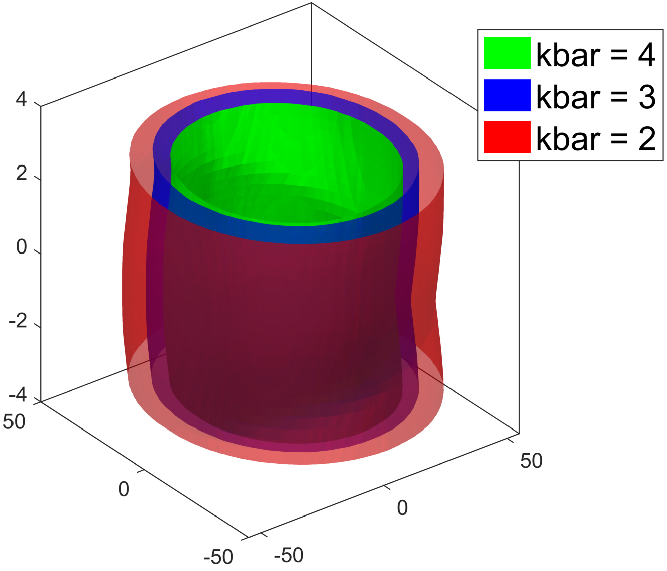
\includegraphics[width=0.6\columnwidth]{figs/bufferRegions_3D}
  \caption{Buffer regions for different $\nva$ (best visualized with colors). As $\nva$ decreases, a larger buffer is required between vehicles to ensure that the intruder spends more time while traveling through this buffer region so that it forces fewer vehicles to apply an avoidance maneuver.}
  \label{fig:buffRegions}
\end{figure}
We also computed the buffer regions for $\nva = 2$ and $\nva = 4$. 
% The results are shown in Figure \ref{fig:buffRegions}. 
%Top-down views of these 3D sets are shown in Figure \ref{fig:buffRegions_td}. 
As shown in Figure \ref{fig:buffRegions}, a bigger buffer is required between vehicles when $\nva$ is smaller. Intuitively, when $\nva$ is smaller, a larger buffer is required to ensure that the intruder spends more time ``traveling" through this buffer region so that it can affect fewer vehicles in the same duration.             
%\begin{figure}[H]
%  \centering
%  \includegraphics[width=0.8\columnwidth]{"figs/bufferRegions_topdown"}
%  \caption{Top-down view of the buffer regions for different $\nva$ shown in Figure {fig:buffRegions} (best visualized with colors). As $\nva$ decreases, $\brd$ increase and a larger buffer is required between vehicles.}
%  \label{fig:buffRegions_td}
%\end{figure}

These buffer region computations along with the induced obstacle computations were similarly performed sequentially for each vehicle to obtain $\obsset(\cdot)$ in \eqref{eq:obsseti_intr}. This overall obstacle set was then used during their trajectory planning and the control policy $\ctrl^{\text{PP}}(\cdot)$ was computed, as defined in \eqref{eqn:PPPolicy}. Finally, the corresponding nominal trajectories were obtained by executing control policy $\ctrl^{\text{PP}}(\cdot)$. %The nominal trajectory thus corresponds to the trajectory that a vehicle will follow if the intruder does not appear in the system. 
The nominal trajectories and the overall obstacles for different vehicles are shown in Figure \ref{fig:trajObsSim}. The numbers in the figure represent the vehicle numbers. The nominal trajectories (solid lines) are well separated from each other to ensure collision avoidance even during a worst-case intruder ``attack". At any given time, the vehicle density is low to ensure that the intruder cannot force more 3 vehicles to apply an avoidance maneuver. This is also evident from large obstacles induced by vehicles for the lower priority vehicles (dashed circles). This lower density of vehicles is the price that we pay for ensuring that the replanning can be done efficiently in real-time. We discuss this further in section \ref{sec:discuss}.
%The dashed circle around a vehicle denote the overall obstacle induced by that vehicle for the lower priority vehicles. As expected, all vehicles are outside each other's induced obstacles, as well as static obstacles. Accounting for this worst-case behavior makes our reachability analysis conservative and this limitation is discussed more Section \ref{sec:discuss}.
\begin{figure}
  \centering
  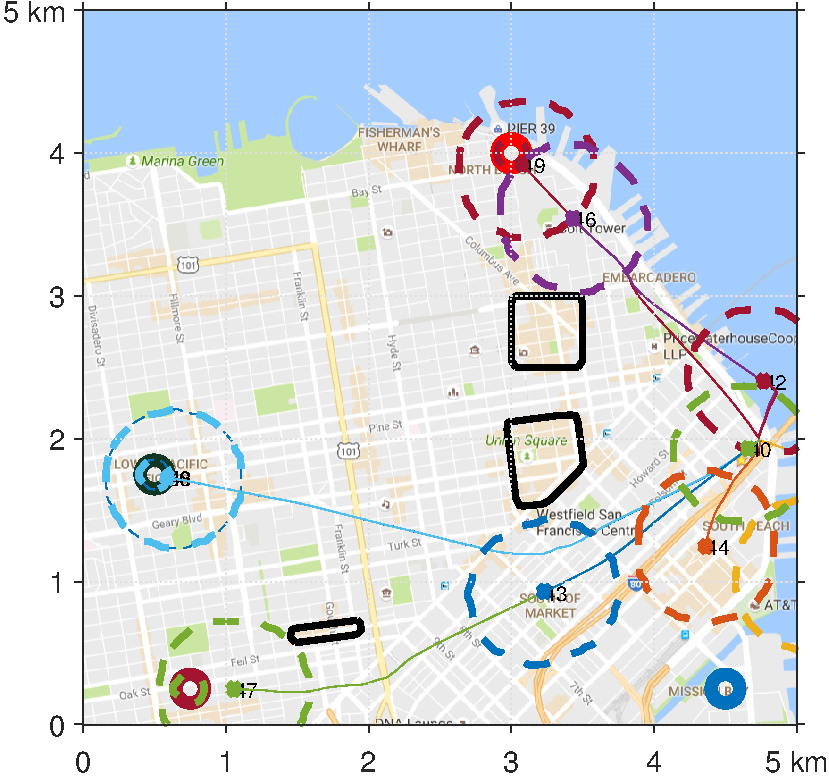
\includegraphics[width=0.8\columnwidth]{figs/nomTraj}
  \caption{Nominal trajectories and induced obstacles by different vehicles. The nominal trajectories (solid lines) are well separated from each other to ensure that the intruder cannot force more than 3 vehicles to apply an avoidance maneuver.}
  \label{fig:trajObsSim}
\end{figure}

In the absence of an intruder the vehicles transit successfully to their destinations with control policy $\ctrl^{\text{PP}}(\cdot)$, but they can deviate from the shown nominal trajectories if an intruder appears in the system. In Figure \ref{fig:trajComparison}, we plot the distance between an STP vehicle and the intruder when the vehicle applies the control policy $\ctrl^{\text{PP}}(\cdot)$ (Red line) vs when it applies ${\ctrl^{\text{A}}}$ (Blue line). Black dashed line represents the collision radius $r=$\SI{100}{\m} between the vehicle and the intruder. As evident from the figure, if the vehicle continues to apply the control policy $\ctrl^{\text{PP}}(\cdot)$ in the presence of an intruder, the intruder enters in its danger zone. Thus, it is forced to apply the avoidance control, which can cause a deviation from the nominal trajectory, but will successfully avoid the intruder.
\begin{figure}
  \centering
  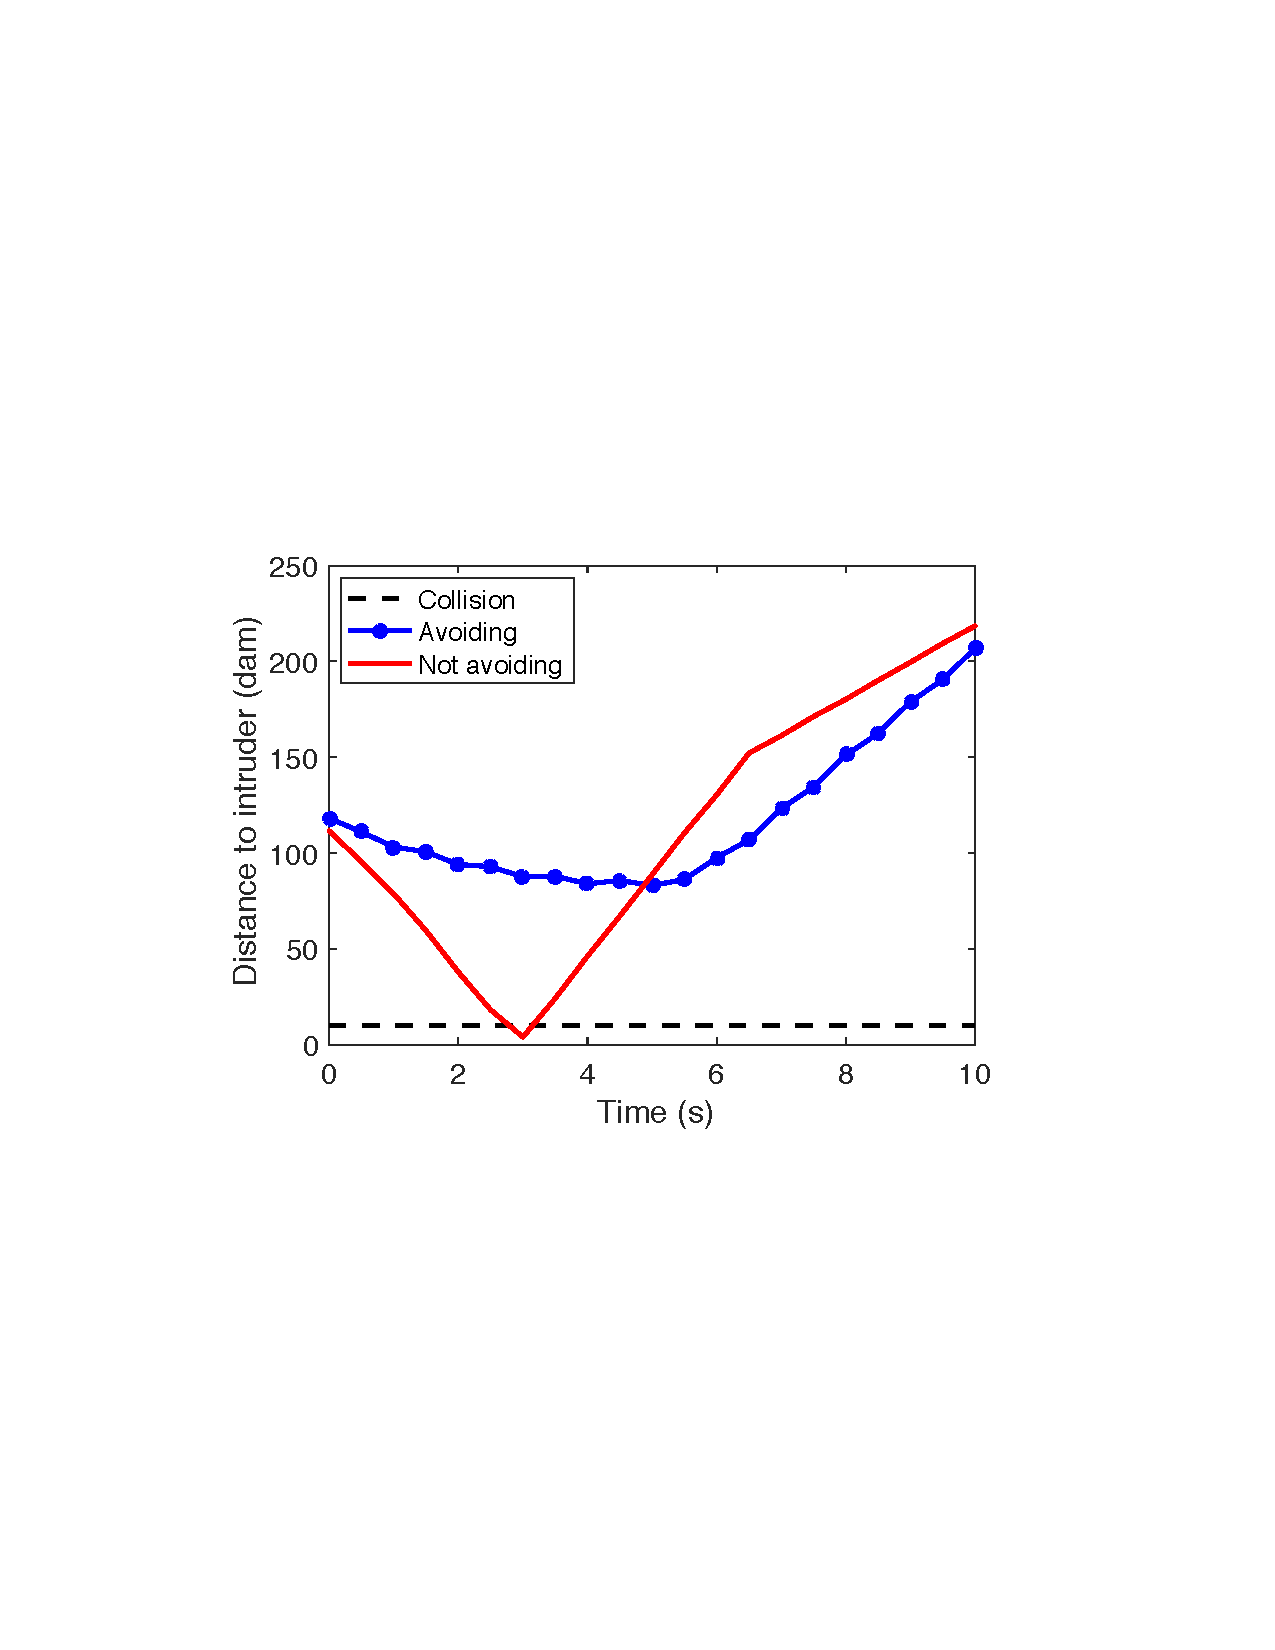
\includegraphics[width=0.6\columnwidth]{figs/simulateIntruder}
  \caption{The trajectory of a STP vehicle when it applies the nominal controller vs when it applies the avoidance control. The vehicle is forced to apply the avoidance maneuver in the presence of an intruder, which can cause vehicle's deviation from its nominal trajectory.}
  \label{fig:trajComparison}
\end{figure}

Under the proposed algorithm, the intruder will affect the maximum number of vehicles ($\nva$ vehicles), when it appears at the boundary of the avoid region of a vehicle, immediately begins travelling through the buffer region between vehicles and reaches the boundary of the avoid region of another vehicle at $\tsa + \brd$ and then the boundary of the avoid region of another vehicle at $\tsa + 2\brd$ and so on. This strategy will make sure that the intruder forces maximum vehicles to apply an avoidance maneuver during a duration of $\iat$. This is illustrated for a small simulation of 4 vehicles in Figure \ref{fig:worstcase}. In this case at $\tsa = 0$, $\veh_{\intr}$ (Black vehicle) appears at the boundary of the avoid region of $\veh_1$ (Blue vehicle) (see Figure \ref{fig:worstcase1}). Immediately, it travels through the buffer region between $\veh_1$ and $\veh_2$ and at $t = \tsa + \brd = $\SI{3.33}{\s}, reaches the boundary of the avoid region of $\veh_2$ (Red vehicle), as shown in Figure \ref{fig:worstcase1}. The trajectories that $\veh_1$ will follow while applying the avoidance control, $\veh_2$ and $\veh_{\intr}$ will follow while trying to collide with each other are also shown. Following the same strategy, $\veh_{\intr}$ reaches the boundary of the avoid region of $\veh_3$ (Green vehicle) at $t = \tsa + 2\brd = $\SI{6.67}{\s}, and will just barely reach the boundary of the avoid region of $\veh_4$ (Pink vehicle) at $t = $\SI{10}{\s}. However, it won't be able to force $\veh_4$ to apply an avoidance maneuver as the duration of $\iat$ will be over by then. Thus the avoid start time of the four vehicles are given as $\tsa_1 = $\SI{0}{\s}, $\tsa_2 = $\SI{3.33}{\s}, $\tsa_3 = $\SI{6.67}{\s} and $\tsa_4 = \infty$. The set of vehicles that will need to replan their trajectories after the intruder disappears is given by $\rvs = \{\veh_1, \veh_2, \veh_3\}$. As expected, $|\rvs| \leq 3$.    
\begin{figure}
\begin{subfigure}{.5\columnwidth}
  \centering
  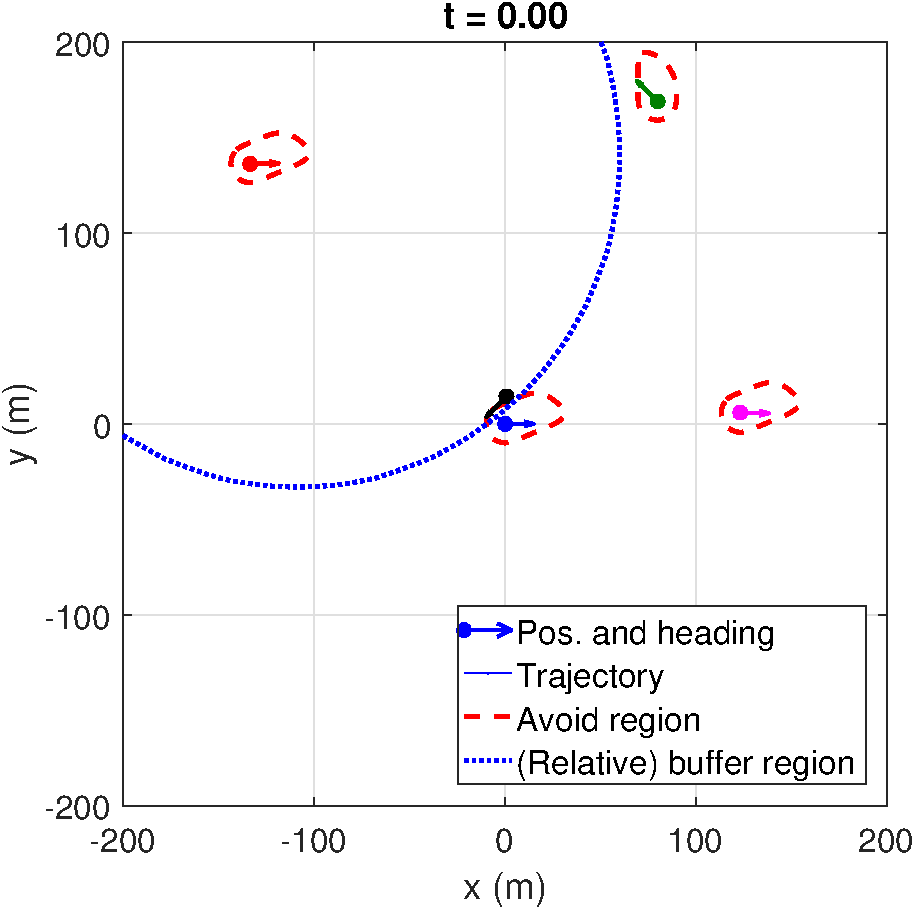
\includegraphics[width=\columnwidth]{figs/simulate_bufferRegion_properties_worst_1}
  \subcaption{}
  \label{fig:worstcase1}
\end{subfigure}%
\begin{subfigure}{.5\columnwidth}
  \centering
  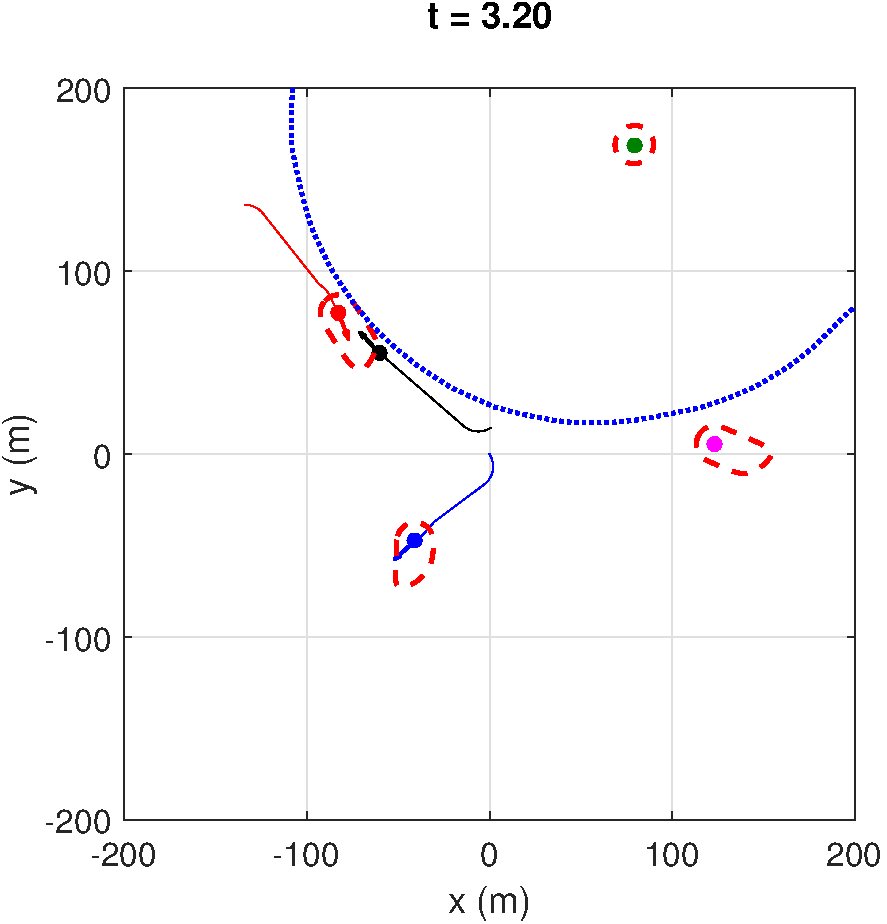
\includegraphics[width=\columnwidth]{figs/simulate_bufferRegion_properties_worst_2}
  \subcaption{}
  \label{fig:worstcase2}
\end{subfigure}
\begin{subfigure}{.5\columnwidth}
  \centering
  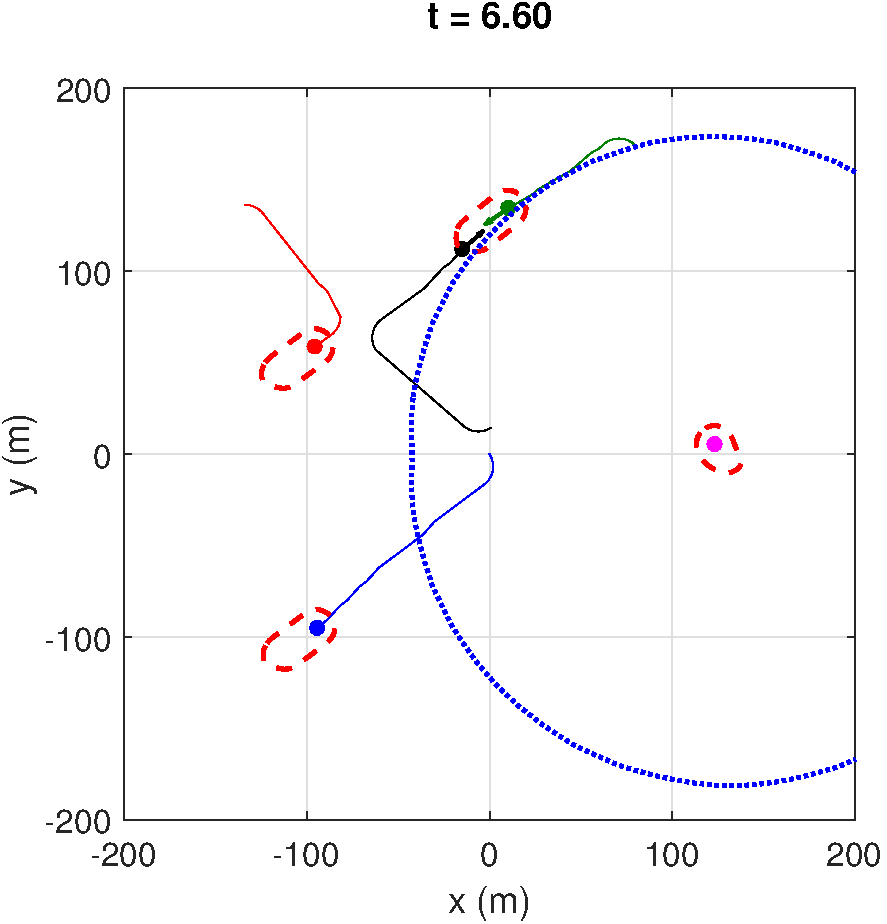
\includegraphics[width=\columnwidth]{figs/simulate_bufferRegion_properties_worst_3}
  \subcaption{}
  \label{fig:worstcase3}
\end{subfigure}%
\begin{subfigure}{.5\columnwidth}
  \centering
  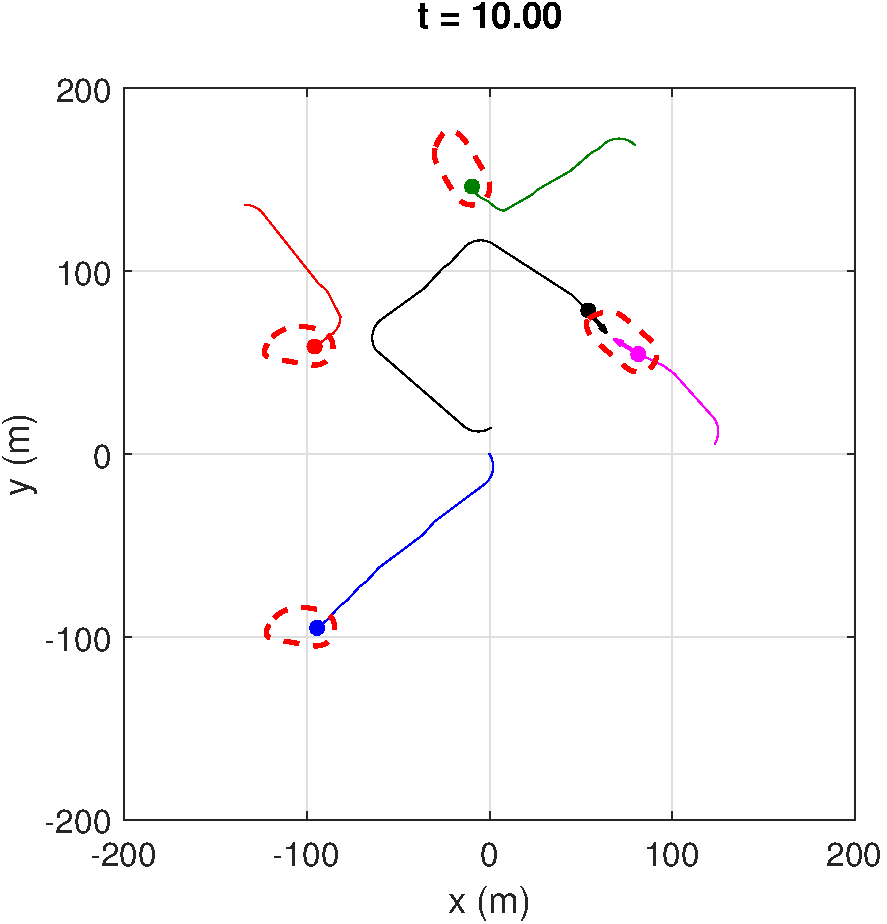
\includegraphics[width=\columnwidth]{figs/simulate_bufferRegion_properties_worst_4}
  \subcaption{}
  \label{fig:worstcase4}
\end{subfigure}
\caption{Illustration of the intruder strategy to force maximum number of vehicles to apply an avoidance maneuver and hence to replan their trajectories. $\veh_{\intr}$ is able to force $\nva=3$ vehicles to apply an avoidance control if the vehicles are applying the worst control which takes it closer to the intruder while the intruder is trying to reach its avoid region boundary. }
\label{fig:worstcase}
\end{figure}

The relative buffer region between vehicles is computed under the assumption that both the STP vehicle and the intruder are trying to collide with each other; this is to ensure that the intruder will need at least a duration of $\brd$ to reach the boundary of the avoid region of the next vehicle, irrespective of the control applied by the vehicle. However, a vehicle will be applying the control policy $\ctrl^{\text{PP}}(\cdot)$ unless the intruder forces it to apply an avoidance maneuver, which may not necessarily correspond to the policy that the vehicle will use to \textit{deliberately} collide with the intruder. Therefore, it is very likely that the intruder will need a larger duration to reach the boundary of the avoid region of next vehicle, and hence it will be able to affect less than $\nva$ vehicles even with its best strategy to affect maximum vehicles. This is also evident from Figure \ref{fig:normalcase}. In this case, $\veh_{\intr}$ again appears at the boundary of the avoid region of $\veh_1$ at $t=0$, as shown in Figure \ref{fig:normalcase1}. The respective targets of the vehicles are also shown. Following its best strategy, the intruder immediately moves to travel through the buffer region between $\veh_1$ and $\veh_2$. However, now $\veh_2$ is applying the control policy $\ctrl^{\text{PP}}(\cdot)$, i.e. it is trying to reach its target, unless the intruder reaches the boundary of its avoid region, which does not happen until $t= $\SI{6.4}{\s}. Now, intruder again tries to travel through the avoid region of $\veh_2$ and $\veh_3$, but is not able to reach the boundary of the avoid region of $\veh_3$ before it is removed from the system at $t=\iat=$\SI{10}{\s}. Thus, the intruder is able to force only two vehicles to apply an avoidance maneuver. The avoid start time of the four vehicles are given as $\tsa_1 = $\SI{0}{\s}, $\tsa_2 = $\SI{6.4}{\s}, $\tsa_3 = \infty$ and $\tsa_4 = \infty$. The set of vehicles that will need to replan their trajectories is given by $\rvs = \{\veh_1, \veh_2\}$. This conservatism in our method is discussed further in Section \ref{sec:discuss}.

The time for planning and replanning for each vehicle is approximately 15 minutes on a MATLAB implementation on a desktop computer with a Core i7 5820K processor. With a GPU-parallelized CUDA implementation in C++ using two GeForce GTX Titan X graphics processing units, this computation time is reduced to approximately 9 seconds per vehicle. So for $\nva = 3$, replanning would take less than 30 seconds. Reachability computations are highly parallelizable, and with more computational resources, replanning should be possible to do within seconds.

\begin{figure}
\centering
\begin{subfigure}{.5\columnwidth}
  \centering
  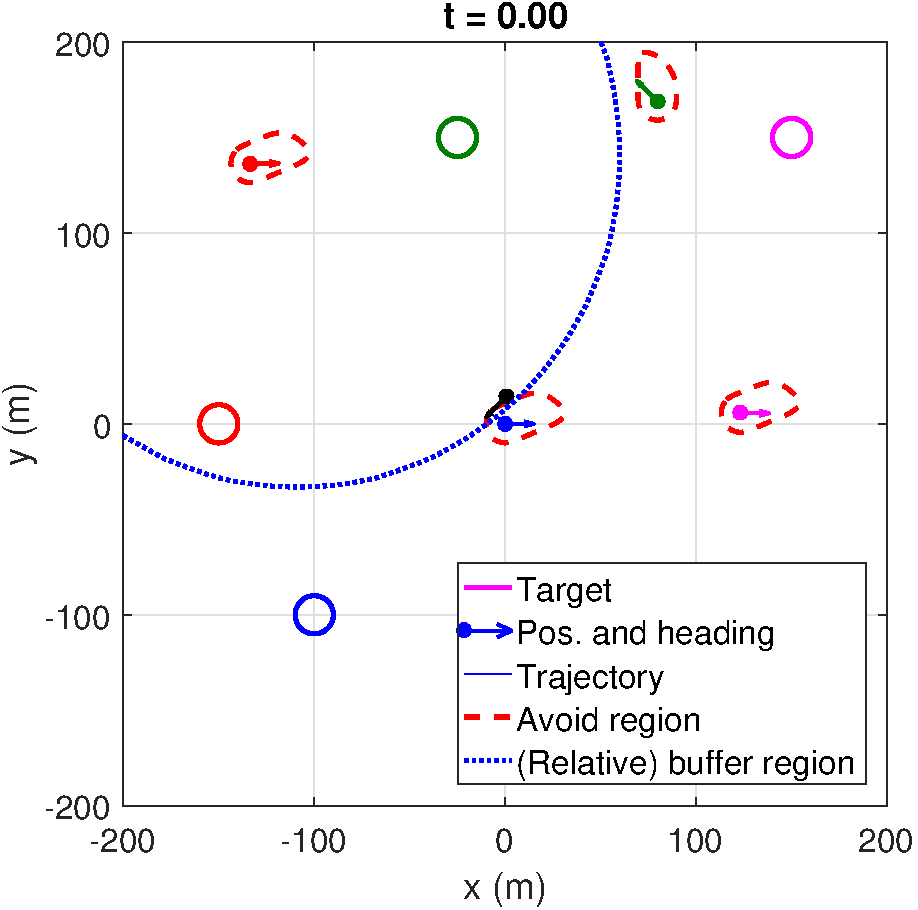
\includegraphics[width=\columnwidth]{figs/simulate_bufferRegion_properties_normal_1}
  \subcaption{}
  \label{fig:normalcase1}
\end{subfigure}%
\begin{subfigure}{.5\columnwidth}
  \centering
  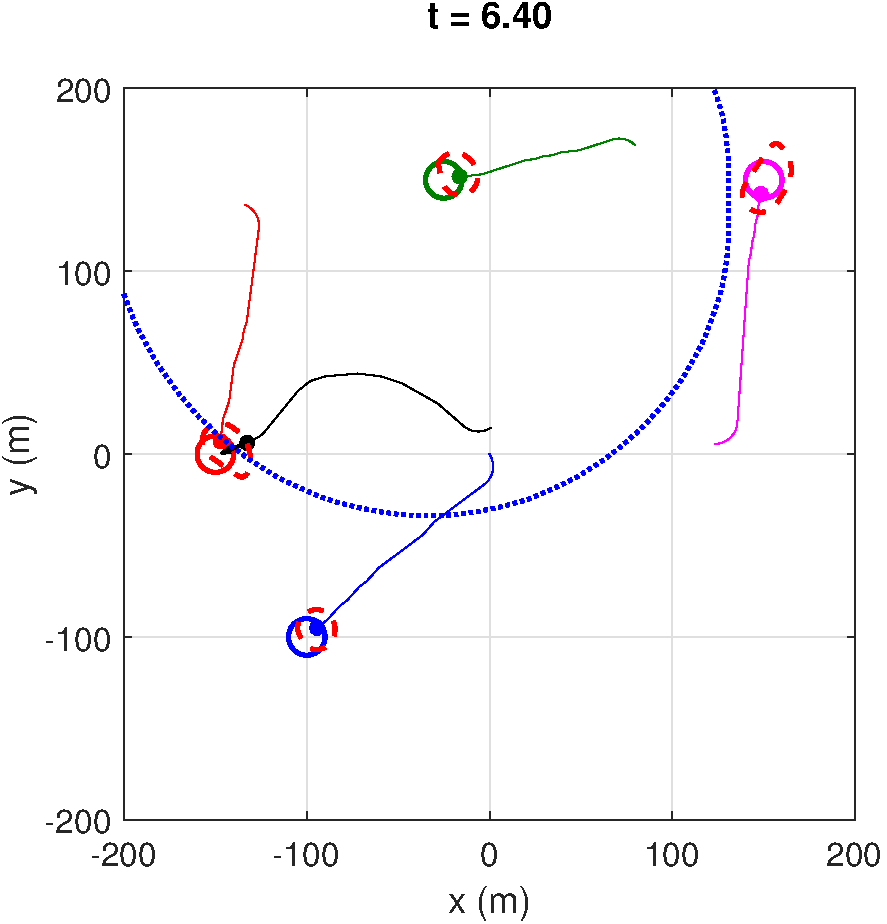
\includegraphics[width=\columnwidth]{figs/simulate_bufferRegion_properties_normal_2}
  \subcaption{}
  \label{fig:normalcase2}
\end{subfigure}
\begin{subfigure}{.5\columnwidth}
  \centering
  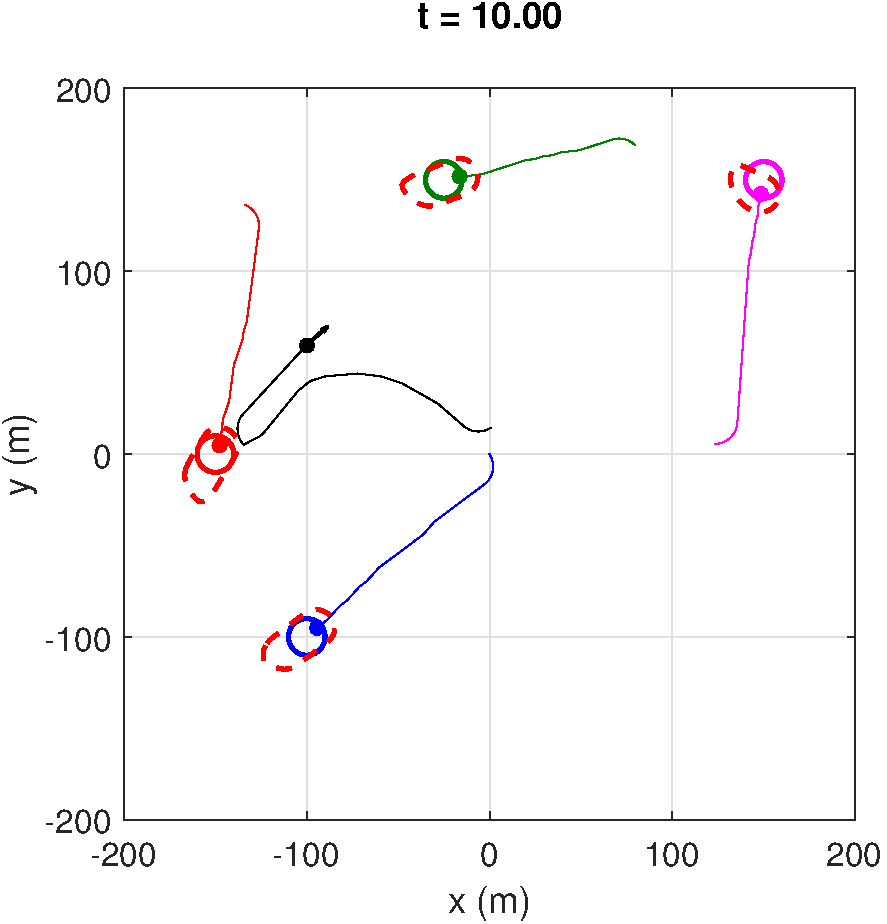
\includegraphics[width=\columnwidth]{figs/simulate_bufferRegion_properties_normal_3}
  \subcaption{}
  \label{fig:normalcase3}
\end{subfigure}%
\caption{Illustration of the intruder strategy to force the maximum number of vehicles to apply an avoidance maneuver and hence to replan their trajectories. Since a vehicle's nominal controller might be different from the worst case controller that is assumed while computing the buffer region, $\veh_{\intr}$ is very likely to be able to force less than $\nva$ vehicles to apply an avoidance maneuver despite its best strategy.}
\label{fig:normalcase}
\end{figure}         

\subsection{Discussion \label{sec:discuss}}
The simulations illustrate the effectiveness of reachability in ensuring that the STP vehicles safely reach their respective destinations even in the presence of an intruder. However, they also highlight some of the conservatism in the worst-case reachability analysis. For example, in the proposed algorithm, we assume the worst-case disturbances and intruder behavior while computing the buffer region and induced obstacles, which results in a large separation between vehicles and hence a lower vehicle density overall, as evident from Figure \ref{fig:trajObsSim}. Similarly, while computing the relative buffer region, we assumed that a vehicle is \textit{deliberately} trying to collide with the intruder so we once again consider the worst-case scenario, even though the vehicle will only be applying the nominal control strategy $\ctrl^{\text{PP}}(\cdot)$, which is usually not be same as the worst-case control strategy. This worst-case analysis is essential to guarantee safety regardless the actions of STP vehicles, the intruder, and disturbances, given no other information about the intruder's intentions and no model of disturbances except for the bounds. However, the conservatism of our results illustrates the need and the utility of acquiring more information about the intruder and disturbances, and of incorporating knowledge of the nominal strategy $\ctrl^{\text{PP}}(\cdot)$, topics that are out of the scope of this paper.